\subsection{Classifications of methods} \label{subject_indexing_types}

% Subject indexing methods can be classified in various manners. For instance, approaches can be classified regarding the origin of the used subjects \cite{golub2019automatic}. Derived \acrshort{si} extracts the subjects from the document itself, while assigned \acrshort{si} maps a fixed set of subjects to the given document.

In this section, we give an overview of the different classifications of \acrshort{si} methods that we have found in the literature. They all revolve around the existence of a \acrfull{kos}, and the availability of training data.

\subsubsection{Golub's classification} \label{subject_indexing_golub}

Golub classifies \acrshort{si} approaches regarding the application purpose, the amount of research backing it and the paradigm used (\acrlong{ml} or string matching, essentially) \cite{golub2019automatic}. It classifies \acrshort{si} approaches into three groups.

\textit{Document clustering} is suited for cases where there is neither training data nor a \acrshort{kos}. Clustering algorithms group documents according to a given similarity metric. They can be used to group documents that belong to the same topic. For example, the similarity metric may measure the amount of mutual information between documents \cite{slonim2002unsupervised}. Document clustering poses two challenges: the resulting structures may be hard to understand \cite{chen2000bringing}, and they can also change once more documents are added. The second challenge is that the assignment of topics to clusters may be unclear and require human intervention.

\textit{Text categorization} is used when both training data and a \acrfull{kos} are available. It consists of a supervised \acrshort{ml} algorithm that learns the features of the subjects of the \acrshort{kos} from the already assigned documents. Once the algorithm is trained, these features will enable it to map subjects to new documents. It can be applied for \acrshort{kos}s that order subjects in hierarchies. Furthermore, doing so may improve the classification accuracy of the method \cite{chen2000bringing}. The third group, \textit{document classification}, is similar to text categorization, but differs from it in the quality of the \acrshort{kos}. The higher \acrshort{kos} quality enables document classification methods to rely on string matching to map subjects to documents, instead of complex machine learning algorithms \cite{khoo2015augmenting}.

\subsubsection{Medelyan's classification} \label{subject_indexing_medelyan}

Medelyan is the author of KEA++ \cite{medelyan2008domain}, a keyphrase extraction algorithm, and also of Maui \cite{medelyan2009human}, another popular indexing algorithm. She differentiates between two types of subject indexing approaches, which she then combines to develop the paradigm used by KEA++.

\textit{Keyphrase extraction} consists of searching for relevant words or phrases in documents. They use solely intrinsic information, such as word frequency or document length. This type of indexing is free in the sense that any keyphrases can be extracted. There is no set of possible keyphrases, i.e. a \acrshort{kos}. The disadvantage of this kind of indexing methods is that the keyphrases won't necessarily have the same form (only words in singular, for example). Also, the presence of undetected synonyms may reduce the quality of the resulting index.

\textit{Term assignment}, on the other hand, uses a \acrshort{kos}. These approaches often rely on string matching to find the keyphrases of the \acrshort{kos} in the documents. The most recent efforts in this field use machine learning methods to map keyphrases to documents. The disadvantage of using classifiers is that they require a lot of training data, whereas string matching method don't require any.

\textit{Keyphrase indexing} combines the two approaches described above, which may be seen as complementary in terms of their strengths and weaknesses. The basic procedure is as follows: given a document, its candidate phrases are first mapped to the keyphrases of the \acrshort{kos} to remove uninformative words and avoid polysemy and synonyms; then, the remaining candidates are analyzed to extract the relevant ones.

In KEA++ \cite{medelyan2008domain}, the analysis of the candidates consists of computing four features for each candidate. These features are fed to a \acrshort{ml} algorithm, which outputs a boolean value stating if the corresponding candidate should be assigned to the document or not. The \acrshort{ml} algorithm is supervised, i.e. it requires a training set. KEA++ uses the Naive Bayes algorithm, which offered the best results when compared with other supervised \acrshort{ml} algorithms like the SVMs and decision trees.

\subsubsection{Töpfer's classification} \label{subject_indexing_toepfer}

Töpfer differentiates between lexical and associative indexing approaches and concludes that both approaches complement each other, which is an argument in favor of fusion architectures, the third member of his classification of \acrshort{si} methods \cite{toepfer2020fusion}. We will look at these three groups in this section.

\textit{Associative approaches} find correlations between words \cite{suominen2019annif} by computing co-occurrence statistics, which allow the methods to identify references to the subjects of the \acrshort{kos}. These methods require training data to learn the mappings. Subjects that do not appear in the training data cannot be assigned to any documents, because the model has not learned weights for them. This means that associative approaches require a lot of training data that is well distributed among the subjects, as it is not able to predict unseen subjects.

\textit{Lexical approaches} map salient terms in the document to the subjects using a trained model \cite{suominen2019annif}. KEA++ \cite{medelyan2008domain}, presented in the previous section, is a lexical approach. Because the weights and the threshold are shared by all subjects, lexical models can be used to assign previously unseen subjects. The parameter estimations are reliable because the values computed for each candidate are usually non-vanishing \cite{toepfer2020fusion}. Therefore, not so much training data is required.

Both approaches may lead to low recall. Associative approaches may have low recall when the training data is insufficient. This is likely to be the case because of \textit{Zipf's law}: when ranked by frequency, the frequency of each subject is half of its predecessor. On the other hand, lexical systems may suffer from low recall when the \acrshort{kos} lacks synonyms, which could hamper the hit rate of the string matching step.

\begin{figure}
    \centering
    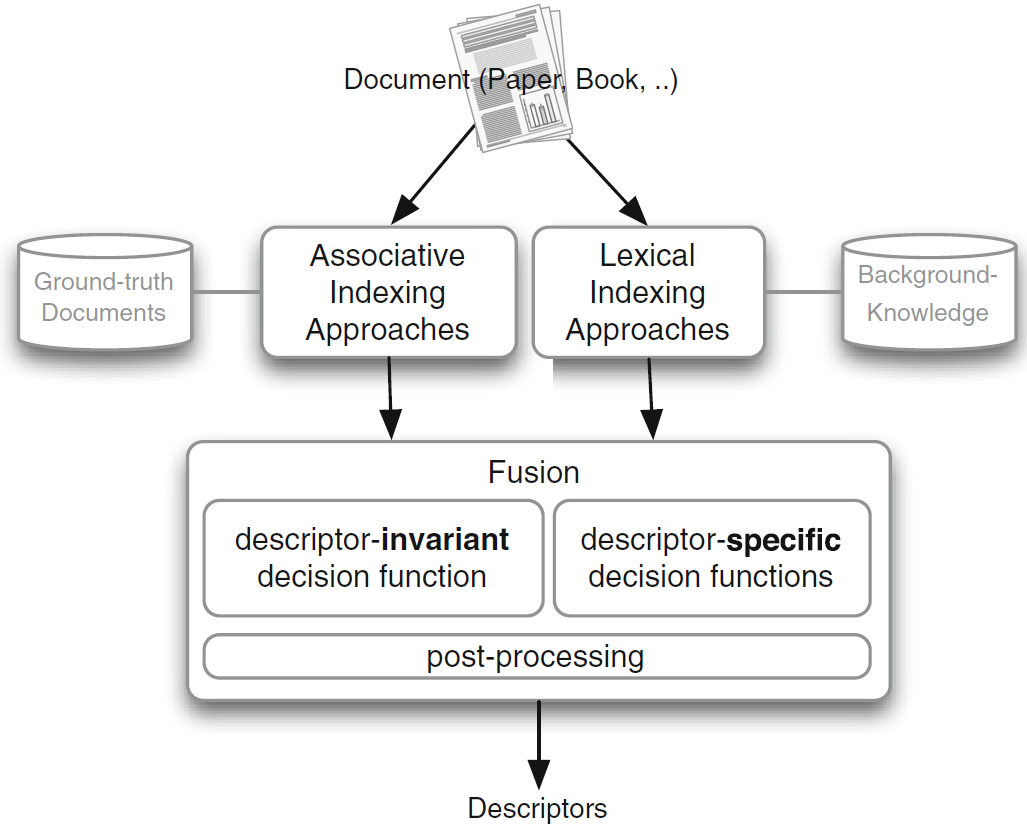
\includegraphics[width=.5\textwidth]{figures/related_work/fusion_architecture.PNG}
    \caption{Schema of a fusion architecture. From \cite{toepfer2020fusion}.}
    \label{fig:fusion_architecture}
\end{figure}

\textit{Fusion architectures} combine lexical and associative indexing systems. Their goal is to gather the advantages of both methods, which were shown to be complementary in the previous section, in one system. Figure \ref{fig:fusion_architecture} shows a schema of the architecture. The decision function, which can be either invariant or specific regarding the subjects, merges the results of the indexing systems into a single set of subjects, which is then assigned to the document after some optional post-processing. The descriptor-invariant decision function may be used for all descriptors, also unseen ones. The descriptor-specific decision function uses the background knowledge and the ground-truth documents to decide on the output.



\subsubsection{Comparison of classifications}

The usage of a \acrshort{kos} and the requirement of training data are the two distinguishing factors of the classifications. These are summarized in table \ref{tab:subject_indexing_classifications}. We will now look at them as a whole and establish relationships between them when possible.

\begin{table}
\centering
\begin{tabular}{|c|c|c|c|c|}
\hline
\thead{Author} & \thead{Group} & \thead{KOS} & \thead{Tr. data} & \thead{Method} \\
\hline\hline
\multirow{3}{*}{Golub} & Text categorization & Yes & Yes & ML algorithm \\ \cline{2-5}
& Document clustering & No & No & ML algorithm \\ \cline{2-5}
& Document classification & Yes & No & String matching \\ \cline{2-5}
\hline
\multirow{3}{*}{Medelyan} & Keyphrase extraction & No & No & String matching \\ \cline{2-5}
& Term assignment & Yes & Yes & Any \\ \cline{2-5}
& Keyphrase indexing & Yes & Yes & ML algorithm \\ \cline{2-5}
\hline
\multirow{3}{*}{Töpfer} & Associative methods & Yes & Yes & ML algorithm \\ \cline{2-5}
& Lexical methods & Yes & Yes & Both \\ \cline{2-5}
& Fusion architecture & Yes & Yes & Both \\ \cline{2-5}
\hline
\end{tabular}
\caption{Summary of the SI classifications.}
\label{tab:subject_indexing_classifications}
\end{table}

Golub's \textit{document clustering} and Medelyan's \textit{keyphrase extraction} are the only categories that require neither a \acrshort{kos} nor assigned documents as training data. They differ mainly in their objective: document clustering focuses on the subjects that relate documents, whereas keyphrase extraction looks at each document individually, looking for its most significant subjects.

Töpfer mentions Medelyan's models (KEA++ \cite{medelyan2008domain} and Maui \cite{medelyan2009human}) as examples of \textit{lexical methods}. Given that, according to Medelyan's classification, they belong to the \textit{keyphrase indexing} category, we can establish a relationship among these two categories. Furthermore, \textit{keyphrase indexing} arises from combining the other two categories of Medelyan's classification (\textit{term assignment} and \textit{keyphrase extraction}). Therefore, all three categories from Medelyan can be placed under Töpfer's lexical methods. Golub's \textit{text categorization} also requires training data and a \acrshort{kos}, and uses an \acrshort{ml} algorithm as well.

Finally, Medelyan mentions that \textit{term assignment} methods only require training data if an \acrshort{ml} algorithm is going to be used. If string matching is used, no training data is required. In this case, \textit{term assignment} would be equivalent to Golub's \textit{document classification} category, where the \acrshort{kos} is expected to be large enough for its entries to appear verbatim in the documents.

Considering all these similarities, we can identify three main types of \acrshort{si} methods. Those that require neither training data nor a \acrshort{kos}, those that only require a \acrshort{kos} and those that require both a \acrshort{kos} and training data.